\documentclass[a4paper,11pt,titlepage]{article}
 
\usepackage[utf8]{inputenc}
\usepackage[spanish]{babel}
\usepackage[T1]{fontenc}
\usepackage{lmodern}
\usepackage{float}
 
\usepackage{parskip}
\usepackage{graphicx}
\usepackage{xcolor}
 
\definecolor{gris}{RGB}{220,220,220}
 
\begin{document}
\begin{titlepage}
  \vspace*{4cm}
  {\fontsize{28}{34}\selectfont\bfseries Antenas de telefonía móvil}
  \par
  \vspace{0.5cm}
  \centering
  % Logo
  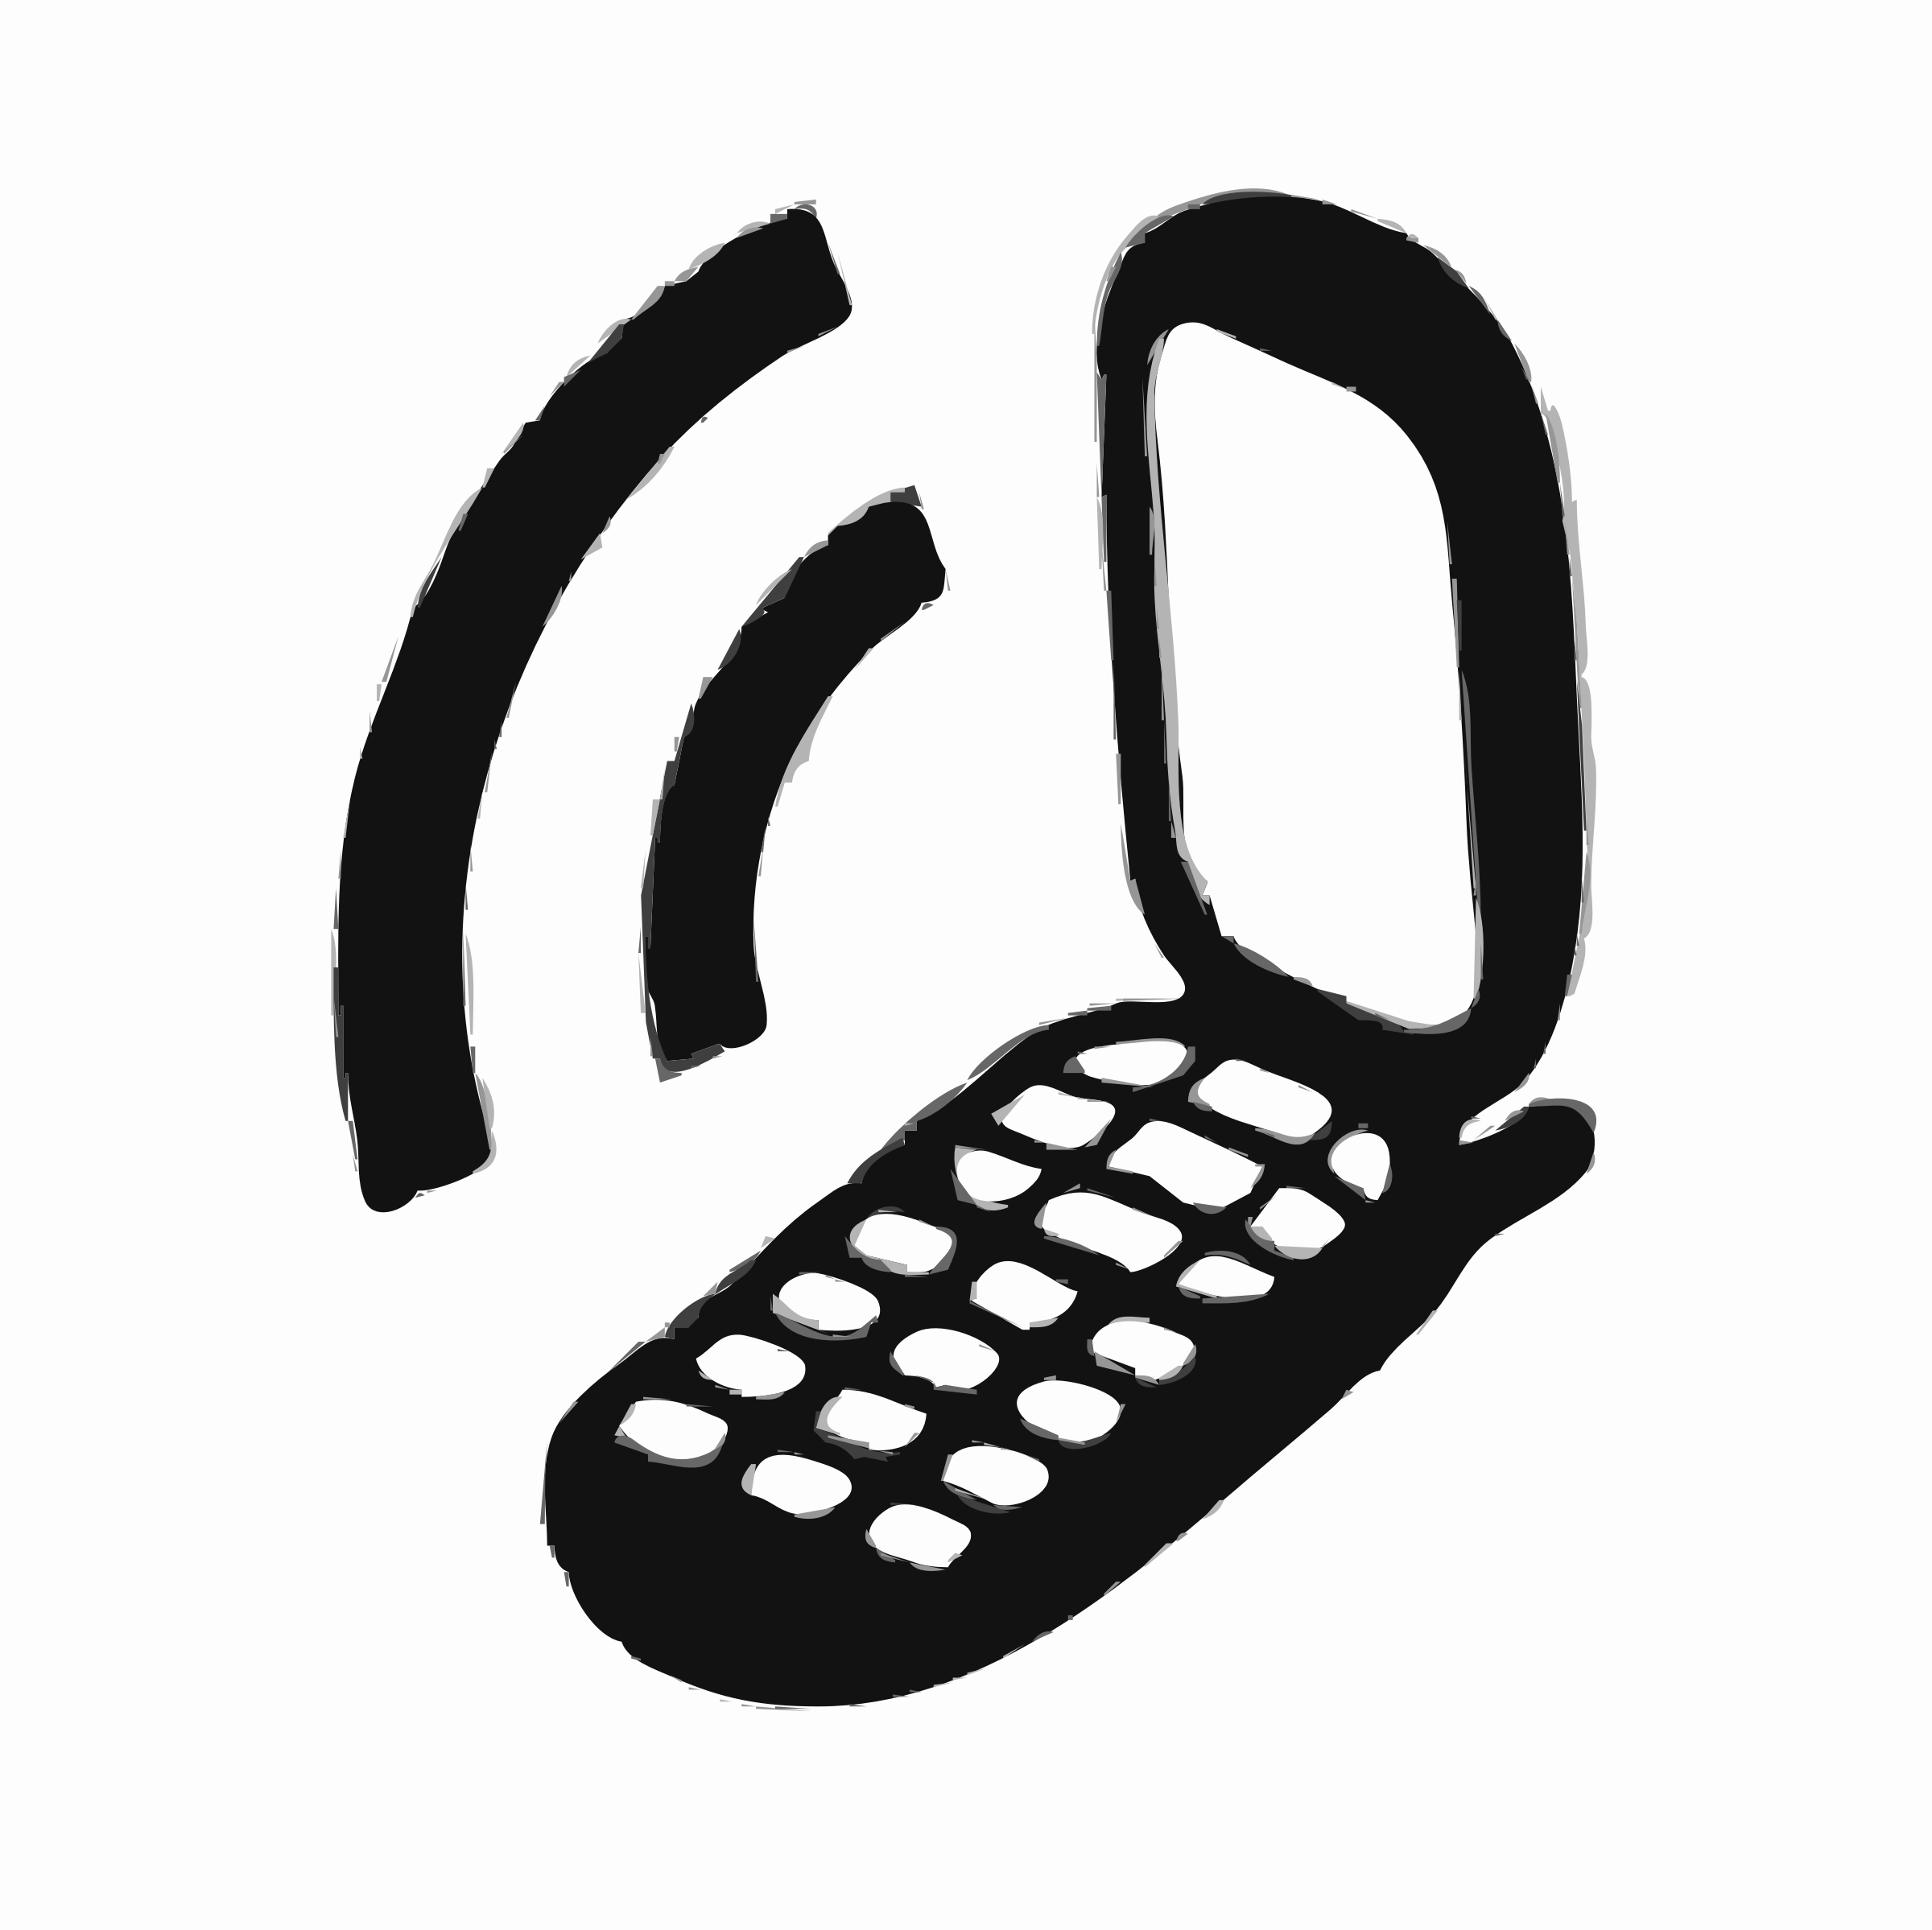
\includegraphics[height=3cm]{movilportada} \\
  % Línea gris
  \vspace{0.5cm}
  {\color{gris}\hrule}
  \Large{\itshape Radiación y propagación electromagnéticas}
  \vfill
  {\large Manuel de la Cruz González \hfill Abril 2019}
\end{titlepage}
\tableofcontents
\newpage
%EVOLUCION
\section{Evolución de las antenas de teléfonos móviles}
%GEN CERO
\subsection{Generación cero o radio-móvil}
Esta generación recibe el nombre de precelular ya que es anterior a la generación de teléfonos móviles. \par
Los radio-móviles se diferencian de los radioteléfonos (walkie-talkie) en que la tecnología que utilizaban estaba disponible como servicio comercial conectado a la red de telefonía pública, mientras que los walkie talkie y demás sistemas de radioafición son independentes de la red de telefonía.\par
\begin{figure}[h]
\centering
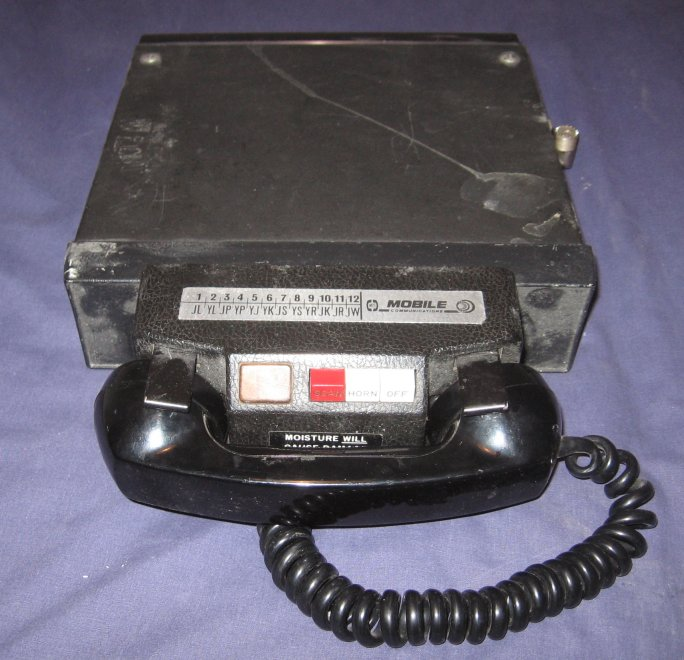
\includegraphics[width=0.5\textwidth]{cero}
\caption{Radio móvil}

\label{imagencero}
\end{figure}
Estos dispositivos se solían utilizar en coches o camiones, llegando a existir en forma de maletín. Las antenas eran externas y estaban situadas en el vehículo donde estaba instalado el radio-móvil.
Este servicio de comunicación comenzó en EEUU en 1946 gracias a la compaía Motorola en unión con Bell System. En Europa comenzaron a usarse en 1952 (República Federal Alemana) y para 1978 (Czechoslovakia) la mayoría de países disponían de este servicio.
%GEN 1
\subsection{Primera Generación o 1G}
Esta generación es la primera de los móviles como los conocemos hoy en día. Esta tecnología analógica comenzó en 1980 y no parói hasta ser sustitutida por el 2G. La principal diferencia entre el 1G y el 2G es que las radio señales que usaban las redes de 1G son analógicas mientras que las de 2G son digitales.\par
La frecuencia de trabajo de estos equipos era de 800 Mhz.
El primer equipo portable de antena para un cuarto de onda tenía una longitud de 9.4 cm y era antena única, no un array.
El primer móvil lanzado al mercado fue el Motorola DynaTAC8000X y la antena que utiliza es una "sleeve dipole". Esta antena no se usa en móviles actuales sin embargo, se usa bastante es dispositivos de comunicación LAN.\par
\begin{figure}[h]
\centering
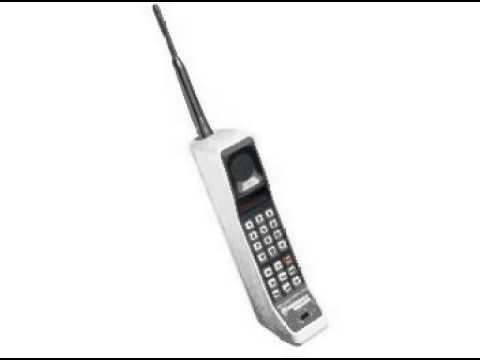
\includegraphics[width=0.6\textwidth]{motorola1}
\caption{Motorola DynaTAC8000X}

\label{motoroladyna}
\end{figure}
Esta antena tiene un consumo eficiente y la longitud se aproximaba a la semilongitud de onda de 850MHz (17 cm).
%GEN 2
\subsection{Segunda Generación o 2G}
En la década de 1990 el 2G trajo varias innovaciones en la telefonía como los servicios de SMS. Se comenzó a operar en GSM 900MHz y más tarde en 1800 MHz.\par
Como ya hemos dicho, su principal diferencia con su predecesora era que ahora este sistema usaba tecnología digital en su network. Esto permitió aumentar la frecuencia y con ello dar más servicios al mismo tiempo.\par
La segunda generación comenzó utilizando únicamente una banda de frecuencia por dispositivo. Así, el Nokia 1011 soportaba sólo GSM900 mientras que otros dispositivos como el Motorola m300 utilizaban GSM1800.\par
Estos teléfono utilizaban dos antenas de monopolo.
\begin{figure}[b]
\centering
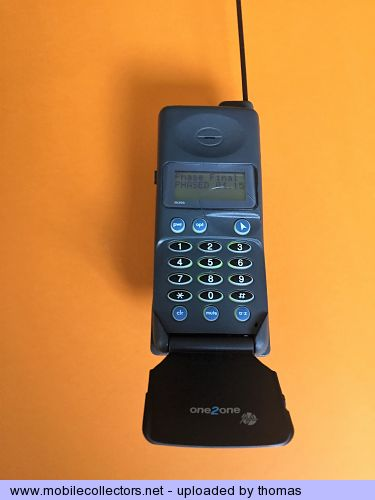
\includegraphics[width=0.6\textwidth]{motorolam300}
\caption{Motorola m300 funcionaba sólo en GSM1800}
\label{motorolam300}
\end{figure}
\par
En 1997, Motorola sacó al mercado el mr601 que fue el primer móvil con dual band. Soportaba tanto GSM1800 como GSM900. Su antena consistía en dos antenas helicoidales cuya forma de onda era de sacacorchos con polarización circular y cuya antena podía ser considerada como tipo dipolo, con patrón de radiación omnidireccional.
\begin{figure}[h]
\centering
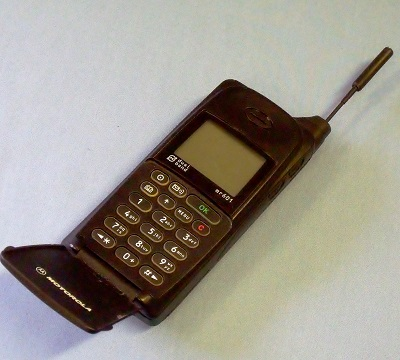
\includegraphics[width=0.6\textwidth]{motorolamr601}
\caption{Motorola mr601}
\label{motorolamr601}
\end{figure}
%FIN
\end{document}